% This is "sig-alternate.tex" V2.1 April 2013
% This file should be compiled with V2.5 of "sig-alternate.cls" May 2012
%
% This example file demonstrates the use of the 'sig-alternate.cls'
% V2.5 LaTeX2e document class file. It is for those submitting
% articles to ACM Conference Proceedings WHO DO NOT WISH TO
% STRICTLY ADHERE TO THE SIGS (PUBS-BOARD-ENDORSED) STYLE.
% The 'sig-alternate.cls' file will produce a similar-looking,
% albeit, 'tighter' paper resulting in, invariably, fewer pages.
%
% ----------------------------------------------------------------------------------------------------------------
% This .tex file (and associated .cls V2.5) produces:
%       1) The Permission Statement
%       2) The Conference (location) Info information
%       3) The Copyright Line with ACM data
%       4) NO page numbers
%
% as against the acm_proc_article-sp.cls file which
% DOES NOT produce 1) thru' 3) above.
%
% Using 'sig-alternate.cls' you have control, however, from within
% the source .tex file, over both the CopyrightYear
% (defaulted to 200X) and the ACM Copyright Data
% (defaulted to X-XXXXX-XX-X/XX/XX).
% e.g.
% \CopyrightYear{2007} will cause 2007 to appear in the copyright line.
% \crdata{0-12345-67-8/90/12} will cause 0-12345-67-8/90/12 to appear in the copyright line.
%
% ---------------------------------------------------------------------------------------------------------------
% This .tex source is an example which *does* use
% the .bib file (from which the .bbl file % is produced).
% REMEMBER HOWEVER: After having produced the .bbl file,
% and prior to final submission, you *NEED* to 'insert'
% your .bbl file into your source .tex file so as to provide
% ONE 'self-contained' source file.
%
% ================= IF YOU HAVE QUESTIONS =======================
% Questions regarding the SIGS styles, SIGS policies and
% procedures, Conferences etc. should be sent to
% Adrienne Griscti (griscti@acm.org)
%
% Technical questions _only_ to
% Gerald Murray (murray@hq.acm.org)
% ===============================================================
%
% For tracking purposes - this is V2.0 - May 2012

\documentclass{sig-alternate-05-2015}
\usepackage[ngerman]{babel}
\usepackage[T1]{fontenc}
\usepackage[utf8]{inputenc}
\usepackage{color}
\usepackage{wrapfig}
\usepackage{graphicx}
\usepackage[listformat=simple]{subcaption}
\usepackage{hyperref}


\begin{document}

% Copyright
\setcopyright{acmcopyright}

\title{Implementierung der {\ttlit Cut \& Count}-Technik für das Feedback Vertex Cover - Problem}
\numberofauthors{2}
\author{
% 1st. author
\alignauthor
Levin von Hollen\\
       \affaddr{Institut für Informatik}\\
       \affaddr{Technische Fakultät}\\
       \affaddr{Christian-Albrechts Universität Kiel}\\
% 2nd. author
\alignauthor
Tilman Beck\\
       \affaddr{Institut für Informatik}\\
       \affaddr{Technische Fakultät}\\
       \affaddr{Christian-Albrechts Universität Kiel}\\
}

\maketitle
\begin{abstract}
Abstract
\end{abstract}

\keywords{Cut\&Count; Feedback Vertex Cover; Nice Tree Decomposition; Python}

\section{Introduction}
Introduction

\section{Nice Tree Decomposition}
what is a tree decomposition?why do we need it?differences to NTD?
\subsection{Representation of Tree Decomposition}
how do we represent in python the ntd, our data structure
\subsection{From Tree Decomposition to Nice Tree Decomposition}
algorithm-steps from TD to NTD

\section{Steiner Tree}
short explanation of problem
implementation of cut \& count on steiner tree

You can use whatever symbols, accented characters, or
non-English characters you need anywhere in your document;
you can find a complete list of what is
available in the \textit{\LaTeX\
User's Guide}\cite{Lamport:LaTeX}.

\section{Feedback Vertex Cover}
short explanation of problem
Difference to steiner tree
implementation of cut \& count

\subsection{subsection for fvc}
asd

\subsection{Tables}
Because tables cannot be split across pages, the best
placement for them is typically the top of the page
nearest their initial cite.  To
ensure this proper ``floating'' placement of tables, use the
environment \textbf{table} to enclose the table's contents and
the table caption.  The contents of the table itself must go
in the \textbf{tabular} environment, to
be aligned properly in rows and columns, with the desired
horizontal and vertical rules.  Again, detailed instructions
on \textbf{tabular} material
is found in the \textit{\LaTeX\ User's Guide}.

Immediately following this sentence is the point at which
Table 1 is included in the input file; compare the
placement of the table here with the table in the printed
dvi output of this document.

\begin{table}
\centering
\caption{Frequency of Special Characters}
\begin{tabular}{|c|c|l|} \hline
Non-English or Math&Frequency&Comments\\ \hline
\O & 1 in 1,000& For Swedish names\\ \hline
$\pi$ & 1 in 5& Common in math\\ \hline
\$ & 4 in 5 & Used in business\\ \hline
$\Psi^2_1$ & 1 in 40,000& Unexplained usage\\
\hline\end{tabular}
\end{table}

To set a wider table, which takes up the whole width of
the page's live area, use the environment
\textbf{table*} to enclose the table's contents and
the table caption.  As with a single-column table, this wide
table will ``float" to a location deemed more desirable.
Immediately following this sentence is the point at which
Table 2 is included in the input file; again, it is
instructive to compare the placement of the
table here with the table in the printed dvi
output of this document.


\begin{table*}
\centering
\caption{Some Typical Commands}
\begin{tabular}{|c|c|l|} \hline
Command&A Number&Comments\\ \hline
\texttt{{\char'134}alignauthor} & 100& Author alignment\\ \hline
\texttt{{\char'134}numberofauthors}& 200& Author enumeration\\ \hline
\texttt{{\char'134}table}& 300 & For tables\\ \hline
\texttt{{\char'134}table*}& 400& For wider tables\\ \hline\end{tabular}
\end{table*}
% end the environment with {table*}, NOTE not {table}!

\subsection{Figures}
Like tables, figures cannot be split across pages; the
best placement for them
is typically the top or the bottom of the page nearest
their initial cite.  To ensure this proper ``floating'' placement
of figures, use the environment
\textbf{figure} to enclose the figure and its caption.

This sample document contains examples of \textbf{.eps} files to be
displayable with \LaTeX.  If you work with pdf\LaTeX, use files in the
\textbf{.pdf} format.  Note that most modern \TeX\ system will convert
\textbf{.eps} to \textbf{.pdf} for you on the fly.  More details on
each of these is found in the \textit{Author's Guide}.

\begin{figure}
\centering
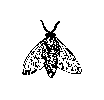
\includegraphics{fly}
\caption{A sample black and white graphic.}
\end{figure}

\begin{figure}
\centering
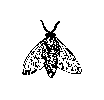
\includegraphics[height=1in, width=1in]{fly}
\caption{A sample black and white graphic
that has been resized with the \texttt{includegraphics} command.}
\end{figure}


As was the case with tables, you may want a figure
that spans two columns.  To do this, and still to
ensure proper ``floating'' placement of tables, use the environment
\textbf{figure*} to enclose the figure and its caption.
and don't forget to end the environment with
{figure*}, not {figure}!

\begin{figure*}
\centering
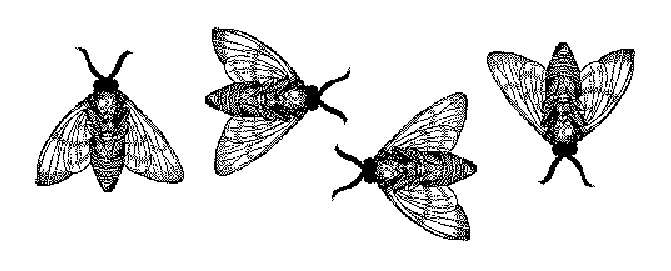
\includegraphics{flies}
\caption{A sample black and white graphic
that needs to span two columns of text.}
\end{figure*}


\begin{figure}
\centering
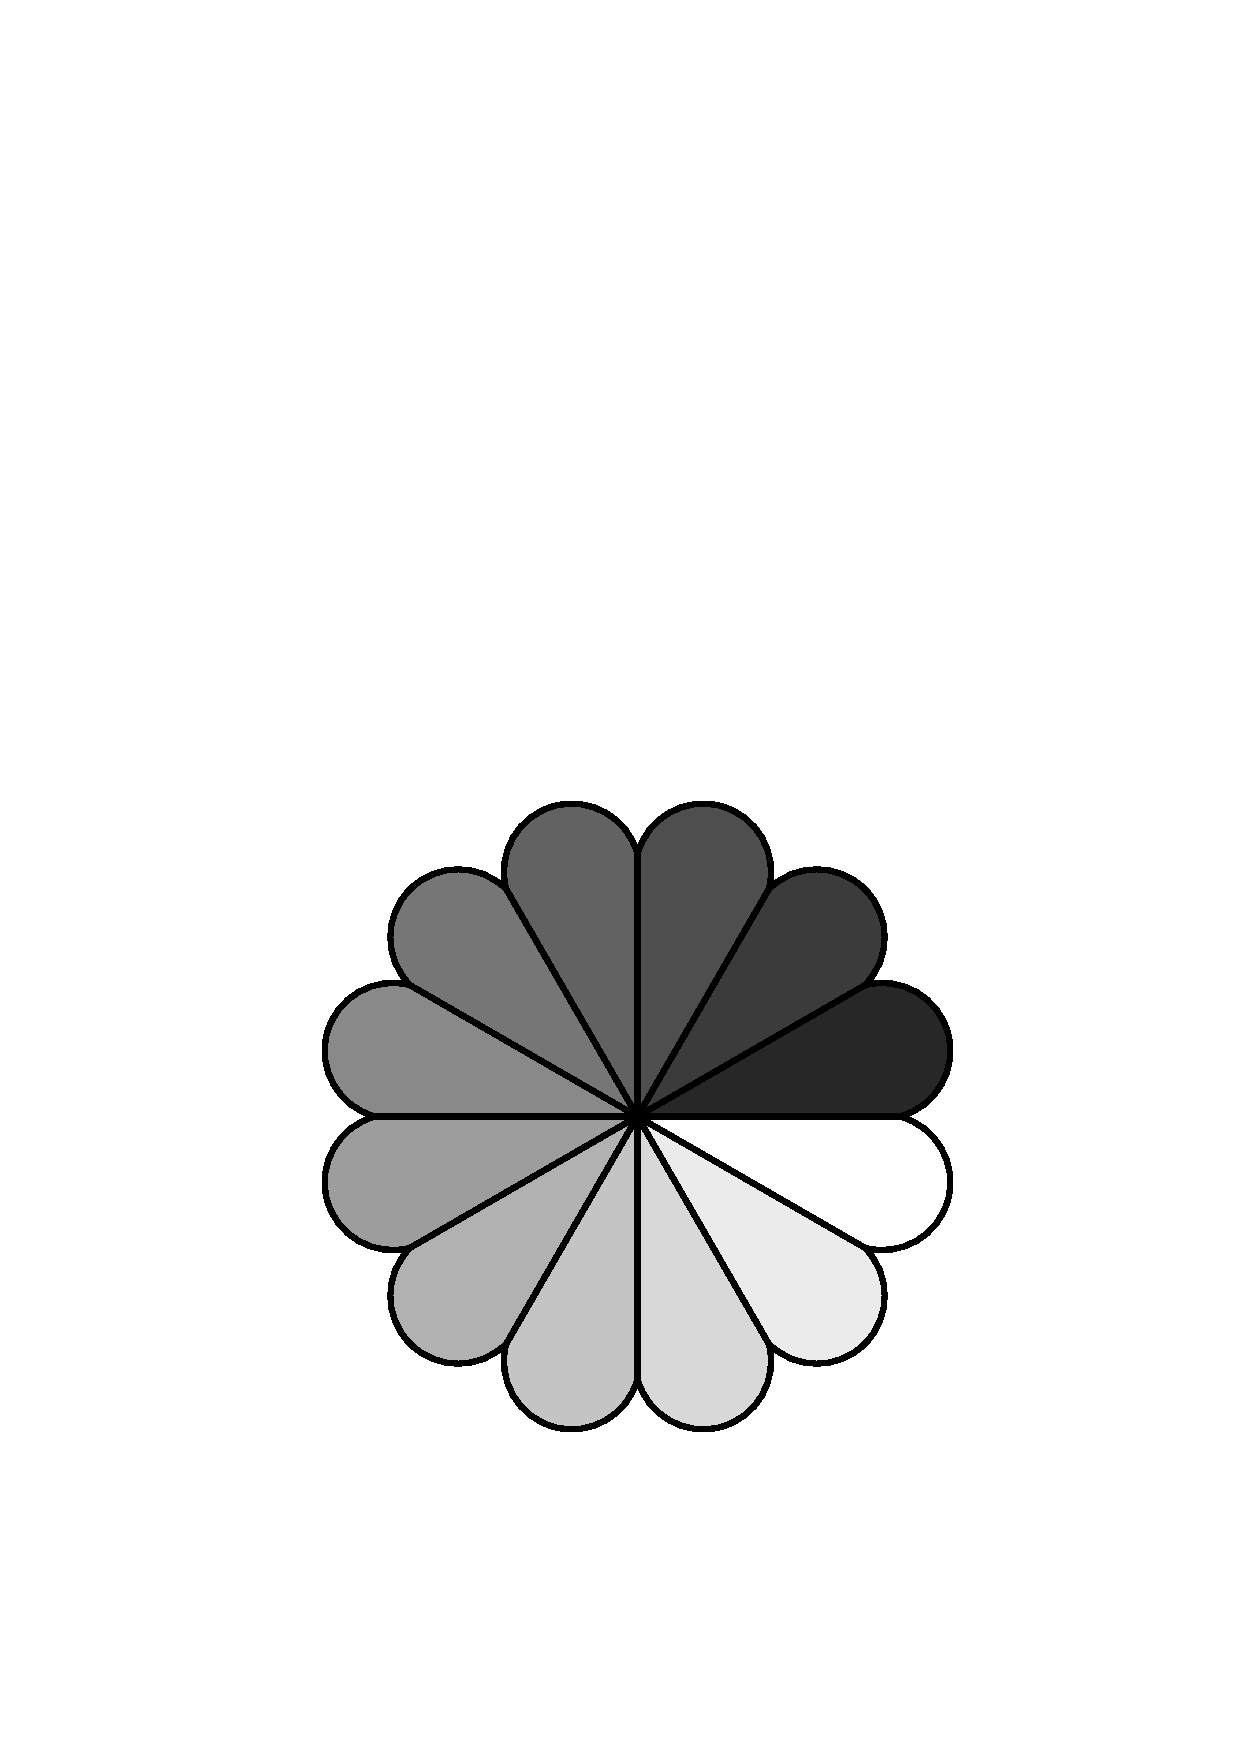
\includegraphics[height=1in, width=1in]{rosette}
\caption{A sample black and white graphic that has
been resized with the \texttt{includegraphics} command.}
\vskip -6pt
\end{figure}

\subsection{Theorem-like Constructs}
Other common constructs that may occur in your article are
the forms for logical constructs like theorems, axioms,
corollaries and proofs.  There are
two forms, one produced by the
command \texttt{{\char'134}newtheorem} and the
other by the command \texttt{{\char'134}newdef}; perhaps
the clearest and easiest way to distinguish them is
to compare the two in the output of this sample document:

This uses the \textbf{theorem} environment, created by
the\linebreak\texttt{{\char'134}newtheorem} command:
\newtheorem{theorem}{Theorem}
\begin{theorem}
Let $f$ be continuous on $[a,b]$.  If $G$ is
an antiderivative for $f$ on $[a,b]$, then
\begin{displaymath}\int^b_af(t)dt = G(b) - G(a).\end{displaymath}
\end{theorem}

The other uses the \textbf{definition} environment, created
by the \texttt{{\char'134}newdef} command:
\newdef{definition}{Definition}
\begin{definition}
If $z$ is irrational, then by $e^z$ we mean the
unique number which has
logarithm $z$: \begin{displaymath}{\log e^z = z}\end{displaymath}
\end{definition}

Two lists of constructs that use one of these
forms is given in the
\textit{Author's  Guidelines}.
 
There is one other similar construct environment, which is
already set up
for you; i.e. you must \textit{not} use
a \texttt{{\char'134}newdef} command to
create it: the \textbf{proof} environment.  Here
is a example of its use:
\begin{proof}
Suppose on the contrary there exists a real number $L$ such that
\begin{displaymath}
\lim_{x\rightarrow\infty} \frac{f(x)}{g(x)} = L.
\end{displaymath}
Then
\begin{displaymath}
l=\lim_{x\rightarrow c} f(x)
= \lim_{x\rightarrow c}
\left[ g{x} \cdot \frac{f(x)}{g(x)} \right ]
= \lim_{x\rightarrow c} g(x) \cdot \lim_{x\rightarrow c}
\frac{f(x)}{g(x)} = 0\cdot L = 0,
\end{displaymath}
which contradicts our assumption that $l\neq 0$.
\end{proof}

Complete rules about using these environments and using the
two different creation commands are in the
\textit{Author's Guide}; please consult it for more
detailed instructions.  If you need to use another construct,
not listed therein, which you want to have the same
formatting as the Theorem
or the Definition\cite{salas:calculus} shown above,
use the \texttt{{\char'134}newtheorem} or the
\texttt{{\char'134}newdef} command,
respectively, to create it.

\section{Conclusions}
This paragraph will end the body of this sample document.
Remember that you might still have Acknowledgments or
Appendices; brief samples of these
follow.  There is still the Bibliography to deal with; and
we will make a disclaimer about that here: with the exception
of the reference to the \LaTeX\ book, the citations in
this paper are to articles which have nothing to
do with the present subject and are used as
examples only.
%\end{document}  % This is where a 'short' article might terminate

%
% The following two commands are all you need in the
% initial runs of your .tex file to
% produce the bibliography for the citations in your paper.
\bibliographystyle{abbrv}
\bibliography{sigproc}  % sigproc.bib is the name of the Bibliography in this case
% You must have a proper ".bib" file
%  and remember to run:
% latex bibtex latex latex
% to resolve all references
%
% ACM needs 'a single self-contained file'!
%
\end{document}
